\Cref{cockpit::sec:experiments} made a case for \cockpit as an effective debugging and
tuning tool. To make the library useful in practice, it must also have limited
computational cost. We now show that it is possible to compute all quantities at
reasonable overhead. The user can control the absolute cost along two
dimensions, by reducing the number of instruments, or by reducing their update
frequency.

All benchmark results show \sgd without momentum. \cockpit's quantities,
however, work for generic optimizers and can mostly be used identically without
increased costs. One current exception is \inlinecode{Alpha} which can be
computed more efficiently given the update rule.\sidenote{This is currently
  implemented for vanilla \sgd. Otherwise, \cockpit falls back to a less
  efficient scheme.}

\subsubsection{Complexity Analysis}

Computing more information adds computational overhead, of course. However,
recent work \citep{dangel2020backpack} has shown that first-order information,
like distributional statistics on the batch gradients, can be computed on top of
the mean gradient at little extra cost. Similar savings apply for most
quantities in \Cref{cockpit::tab:overview-quantities}, as they are
\mbox{(non-)linear} transformations of individual gradients. A subset of
\cockpit's quantities also uses second-order information from the Hessian
diagonal. For ReLU networks on a classification task with $C$ classes, the
additional work is proportional to $C$ gradient backpropagations (\ie $C=10$ for
\cifarten, $C=100$ for \cifarhun). Parallel processing can, to some extent,
process these extra backpropagations in parallel without significant overhead.
If this is no longer possible, we can fall back to a Monte Carlo (MC) sampling
approximation, which reduces the number of extra backprop passes to the number
of samples (1 by default).\sidenote{An MC-sampled approximation of the
  Hessian/generalized Gauss-Newton has been used in \Cref{cockpit::fig:showcase}
  to reduce the prohibitively large number of extra backprops on \cifarhun
  ($C=100$).}

While parallelization is possible for the gradient instruments, computing the
maximum Hessian eigenvalue is inherently sequential. Similar to
\citet{yao2020pyhessian}, we use matrix-free Hessian-vector products by
automatic differentiation \citep{pearlmutter1994fast}, where each product's
costs are proportional to one gradient computation. Regardless of the underlying
iterative eigensolver, multiple such products must be queried to compute the
spectral norm (the number depends on the spectral gap to the second-largest
eigenvalue).

\subsubsection{Run Time Benchmark}

\Cref{cockpit::fig:benchmark-instruments} shows the wall-clock computational
overhead for individual instruments (details in
\Cref{cockpit::app:benchmarks}).\sidenote{To improve readability, we exclude
  \inlinecode{HessMaxEV} here, because its overhead is large compared to other
  quantities. Surprisingly, we also observed significant cost for the 2D
  histogram on GPU. It is caused by an implementation bottleneck for histogram
  shapes observed in deep models. We thus also omit \inlinecode{GradHist2d}
  here, as we expect it to be eliminated with future implementations (see
  \Cref{cockpit::app:run-time-benchmarks} for a detailed analysis and further
  benchmarks). Both quantities, however, are part of the benchmark shown in
  \Cref{cockpit::fig:benchmark_heatmap}.} As expected, byproducts are virtually
free, and quantities that rely solely on first-order information add little
overhead (at most roughly 25\,\% on this problem). Thanks to parallelization,
the ten extra backward passes required for Hessian quantities reduce to less
than 100\,\% overhead. Individual overheads also do not simply add up when
multiple quantities are tracked, because quantities relying on the same
information share computations.

\begin{figure*}
  \centering
  \begin{subfigure}[t]{0.6\linewidth}
    \centering
    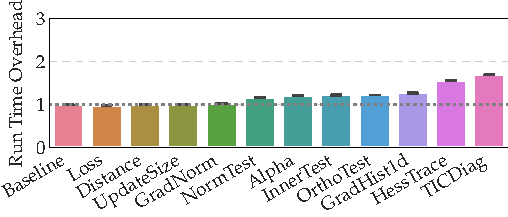
\includegraphics[width=\linewidth]{../repos/cockpit-paper/fig/01_benchmark/output/fig_individual/benchmark_cifar10_3c3d_cuda_thesis-wide}
    \caption{Overhead \cockpit instruments}
    \label{cockpit::fig:benchmark-instruments}
  \end{subfigure}
  \hfill
  \begin{subfigure}[t]{0.35\linewidth}
    \centering
    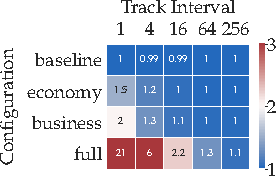
\includegraphics[width=\linewidth]{../repos/cockpit-paper/fig/01_benchmark/output/fig_grid/benchmark_cifar10_3c3d_cuda_thesis-wide}
    \caption{Overhead \cockpit configurations}
    \label{cockpit::fig:benchmark_heatmap}
  \end{subfigure}
  \caption{\textbf{Run time overhead for individual \cockpittitle instruments
      and configurations} as shown on \cifarten \threecthreed on a GPU.
    \subfigref{cockpit::fig:benchmark-instruments} The run time overheads for
    individual instruments are shown as multiples of the \emph{baseline} (no
    tracking). Most instruments add little overhead. This plot shows the
    overhead in one iteration, determined by averaging over multiple iterations
    and random seeds. \subfigref{cockpit::fig:benchmark_heatmap} Overhead for
    different \cockpit configurations. Adjusting the tracking interval and
    re-using the computation shared by multiple instruments can make the
    overhead orders of magnitude smaller. Blue fields mark settings that allow
    tracking without doubling the training time.}
  \label{cockpit::fig:benchmark}
\end{figure*}

To allow a rough cost control, \cockpit currently offers three configurations,
called \inlinecode{``economy''}, \inlinecode{``business''}, and
\inlinecode{``full''}, in increasing order of cost
(\Cref{cockpit::tab:overview-quantities}). As a basic guideline, we consider a
factor of two to be an acceptable limit for the increase in training time and
benchmark the configurations' run times for different tracking intervals.
\Cref{cockpit::fig:benchmark_heatmap} shows a run time matrix for the \cifarten
\threecthreed problem, where settings that meet this limit are set in blue (more
problems including \imagenet are shown in \Cref{cockpit::app:benchmarks}).
Speedups due to shared computations are easy to read off: summing all the
individual overheads shown in \Cref{cockpit::fig:benchmark-instruments} would
result in a total overhead larger than 200\,\%, while the joint overhead
(\textit{business}) reduces to 140\,\%. The \textit{economy} configuration can
easily be tracked at every step of this problem and stay well below our
threshold of doubling the execution time. \cockpit's full view, shown in
\Cref{cockpit::fig:showcase}, can be updated every $64$-th iteration without a
major increase in training time (this corresponds to about five updates per
epoch). Finally, tracking any configuration about once per epoch---which is
common in practice---adds overhead close to zero (rightmost column).

This good performance is largely due to the efficiency of the \backpack package
\citep{dangel2020backpack}, which we leverage with custom and optimized modification,
that compacts information layer-wise and then discards unneeded buffers. Using
layer-wise information (\Cref{cockpit::sec:vanishing_gradient_exp}) scales better to
large networks, where storing the entire model's individual gradients all at
once becomes increasingly expensive (see \Cref{cockpit::app:benchmarks}). To the best of
our knowledge, many of the quantities in \Cref{cockpit::tab:overview-quantities},
especially those relying on individual gradients, have only been explored on
rather small problems. With \cockpit they can now be accessed at a reasonable
rate for deep learning models outside the toy problem category.

%%% Local Variables:
%%% mode: latex
%%% TeX-master: "../thesis"
%%% End:
